\documentclass[a4j,fleqn,dvipdfmx,uplatex]{jsarticle}

\usepackage{sice-si}

\usepackage{epic,eepic}
\usepackage[dvipdfmx]{graphics}
\usepackage[dvipdfmx]{graphicx}
\usepackage[dvipdfmx]{color}
% \usepackage{fancyhdr} % ヘッダフッタの罫線と文字出力
% \pagestyle{fancy} % ヘッダフッタの罫線と文字出力(fancyhdrパッケージとセット)
\usepackage{amsmath} % 数式用
\usepackage{amssymb}
\usepackage{tabularx}
\usepackage{enumerate}
\usepackage{txfonts}
\usepackage{url}
% \usepackage{bm}
\usepackage[subrefformat=parens]{subcaption}
\captionsetup{compatibility=false}

% 図表参照に章番号付加 章をまたいでの参照は不可
\newcommand{\figref}[1]{Fig.\ \ref{#1}}
\newcommand{\tableref}[1]{Table.\ \ref{#1}}

% 章番号の後調整
\newcommand{\secref}[1]{\ref{#1}\hspace{0.2zw} 章}
% 節番号の後調整
\newcommand{\subsecref}[1]{\ref{#1}\hspace{0.2zw} 節}

% 画像挿入テンプレ
% \begin{figure}[tb]
%     \centering
%         \includegraphics[width=\linewidth]{img/〇〇〇〇.jpg}
%         \caption{キャプション}
%         \label{ラベリング}
% \end{figure}


\begin{document}
%
% タイトルと著者名
\title{FTE新入社員課題報告書\\[2mm]社屋屋上室外機における\\散水システム導入および比較検討} % 和文タイトル
\name{○高橋 京佑, 小坂 丞, 仲野 茂翠, 設樂 日和, 𠮷岡 拓海, 渡辺 夏芽, 
\\中村 天音, 塚田 浩貴, 青木 昇, 吉川 唯希, 阪田 悠} % 著者名

\etitle{FTE company building rooftop condensing unit watering system} % 英文タイトル
\ename{\small○KEISUKE Takahashi, TASUKU Kosaka, MOTOAKI Nakano, HINOWA Shidara, TAKUMI Yoshioka, NATSUME Watanabe, \\
AMANE Nakamura, HIROTAKA Tsukada, NOBORU Aoki, ITSUKI Yoshikawa, YU Sakata}	%著者名(英)
%%%%%%%%%%%%%%%%%%%%%%%%%%%%%%%%%%%%%%%%%%%%%%%%%%%%%%%%%%%%%%%%%%%%%%%%%%%%%%%%%%%%%%%%%%%%%%%%%%%
% アブストラクト
\abst
{Recently, "Smart Agriculture" has been promoted in the agricultural sector, but there are issues to be solved in terms of diagnosis technology 
for crop growth and pest invasion. The introduction of multi-spectral sensors will solve these problems. 
"To build a "Spectral Library," we will examine whether it is possible to use UAV to guide flights around the target using "AprilTag."}

% タイトルの出力
\maketitle
%%%%%%%%%%%%%%%%%%%%%%%%%%%%%%%%%%%%%%%%%%%%%%%%%%%%%%%%%%%%%%%%%%%%%%%%%%%%%%%%%%%%%%%%%%%%%%%%%%%
% 本文
\section{序論}\label{sec1}
\subsection{背景}\label{background}
近年, 地球温暖化の影響のため, 日本全国の気温は上昇傾向にあり, 
2021年の大阪府の年間平均気温は1883年に比べ2.5℃上昇している\cite{temp_osaka}. 
さらに, 2021年の真夏日と猛暑日の合計日数は, 2014年の65日に比べ13日増加, 
猛暑日に関しては8日増加しており\cite{temp_osaka2}, 1880年からの真夏日および
猛暑日の長期的推移を見ると増加傾向である (\figref{fig1:temp_osaka}). 

\begin{figure*}[tb]
  \centering
  \begin{minipage}[b]{0.45\linewidth}
      \centering
      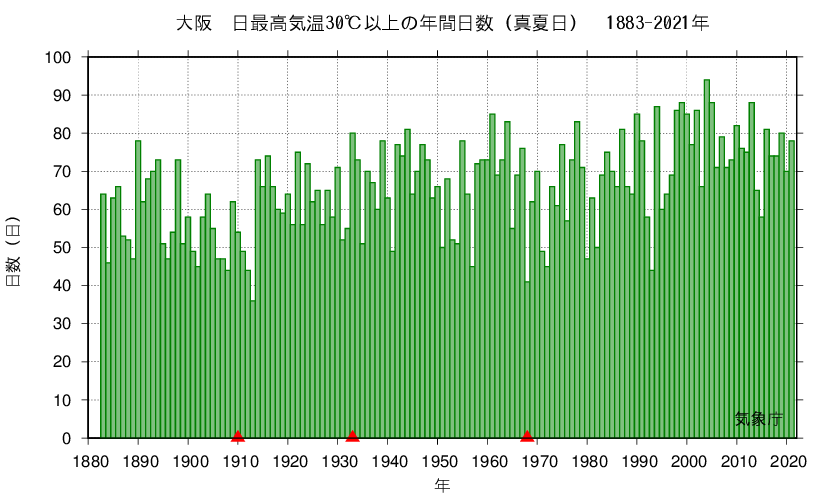
\includegraphics[width=\linewidth]{img/27_OSAKA_tmaxGE30_2021.png}
      \subcaption{大阪 真夏日}
      \label{subfig1:temp_osaka}
    \end{minipage}
    \begin{minipage}[b]{0.45\linewidth}
      \centering
      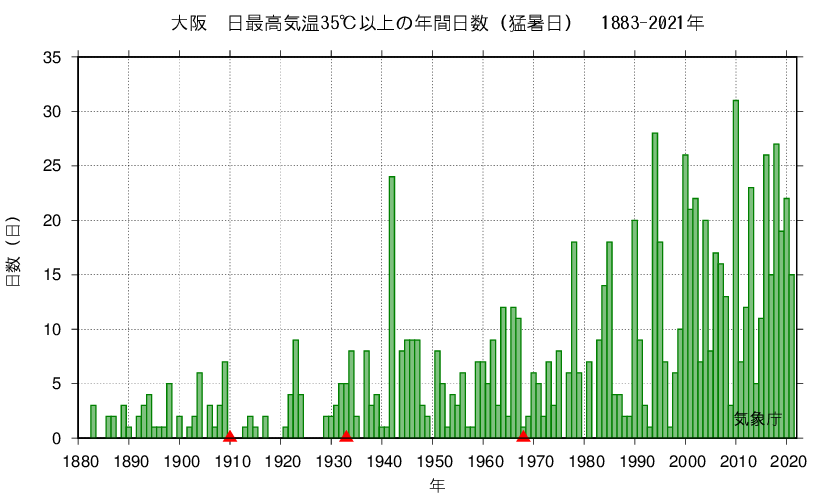
\includegraphics[width=\linewidth]{img/27_OSAKA_tmaxGE35_2021.png}
      \subcaption{大阪 猛暑日}
      \label{subfig1:temp_osaka2}
    \end{minipage}
    \caption{真夏日および猛暑日の年間日数 1883-2021年\cite{temp_osaka3}}
    \label{fig1:temp_osaka}
\end{figure*}
 

空調および冷凍分野において空気を冷やす原理として, "冷凍サイクル" が挙げられる. 
\figref{fig1:cycle}に示す通り, 冷凍サイクルは 「圧縮」「凝縮」「膨張」「蒸発」 
の4行程で構成されている. 冷凍サイクルにおいてモリエル線図(\figref{fig1:ph_r410}) 
は使用する冷媒の状態変化に伴う運転状況の変化, 装置能力, 装置動力などの計算に
よく使用される. 
上記に示した気温上昇に伴い, 今後は空調機の利用機会が増えると予想できる. 一般に
空調機には室内機 (別称: クーラー) と室外機 (別称: 冷凍機) に分類されており, 
冷房時において室外機では「圧縮」と「凝縮」, 室内機では「蒸発」と「膨張」の行程を
それぞれ担っている. 室外機は高圧化した冷媒ガスを外気に熱を伝達することにより凝縮させ, 
室内機では, 膨張した冷媒液を室内の空気と熱交換させて冷媒の潜熱を利用して冷却する. 

\begin{figure}[tb]
  \centering
      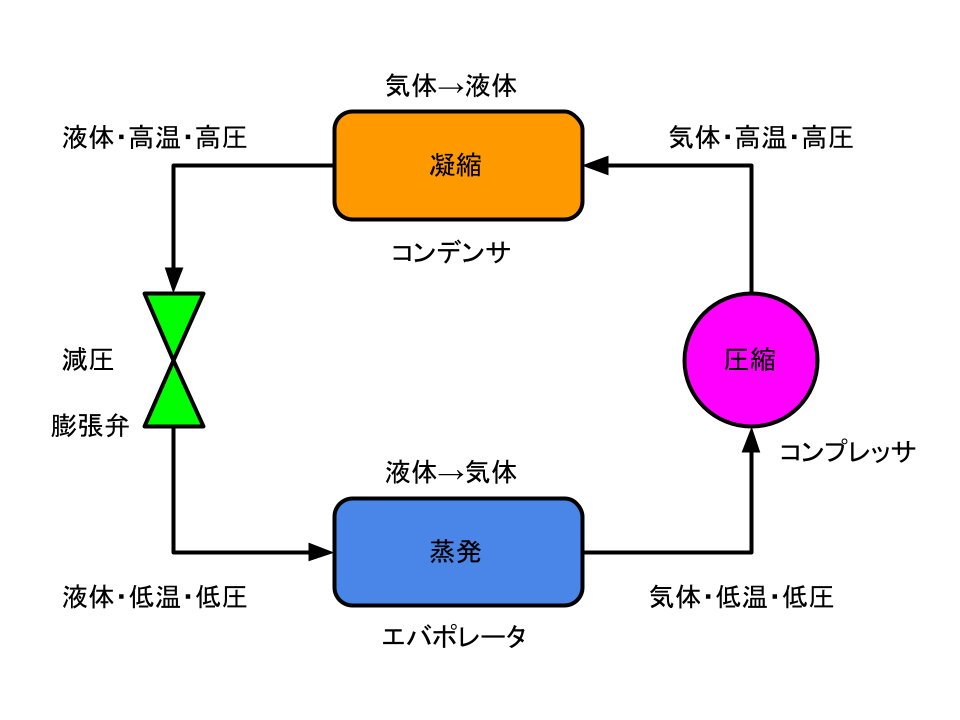
\includegraphics[width=\linewidth]{img/cycle-2.png}
      \caption{冷凍サイクル}
      \label{fig1:cycle}
\end{figure}

\begin{figure}[tb]
    \centering
        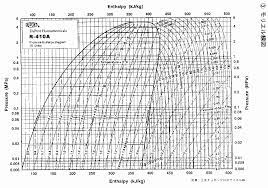
\includegraphics[width=\linewidth]{img/ph線図.jpg}
        \caption{モリエル線図(p-h 線図) 冷媒:R410}
        \label{fig1:ph_r410}
\end{figure}

ここで, 室外機吸い込み側空気, つまり外気温度が上昇すると, それに付随して凝縮温度
が高くなる. それにより冷却能力は小さくなり, 圧縮機駆動の駆動力が大きくなるため, 
成績係数が小さくなる. したがって, 同じ冷凍能力を出すためには消費電力が大きくなる.  
実際に外気温30℃, 相対湿度50\%の環境下で簡易的に10分おきにバケツにて散水をしながら
電力量を計測した. その対照実験の計測環境は\tableref{table:ex1}のとおりである. 

\begin{table}[tbh]
  \caption{計測環境}
  \label{table:ex1}
  \centering
  \begin{tabular}{lcccc}
     & 外気温 & 湿度 & 設定温度 & 気候 \\
    \hline \hline
    実験1 & 34.3 & 48.0 & 27 & 晴れ  \\
    実験2 & 32.9 & 58.9 & 27 & 曇り \\
    \hline
  \end{tabular}
\end{table}

\figref{fig1:compare_watering}に示すように, 実験2 (散水あり) の電力量は実験1 (散水なし) のそれと
比較して小さくなっていることが分かる.

% 散水の有無の電力比較
\begin{figure*}[tb]
  \centering
      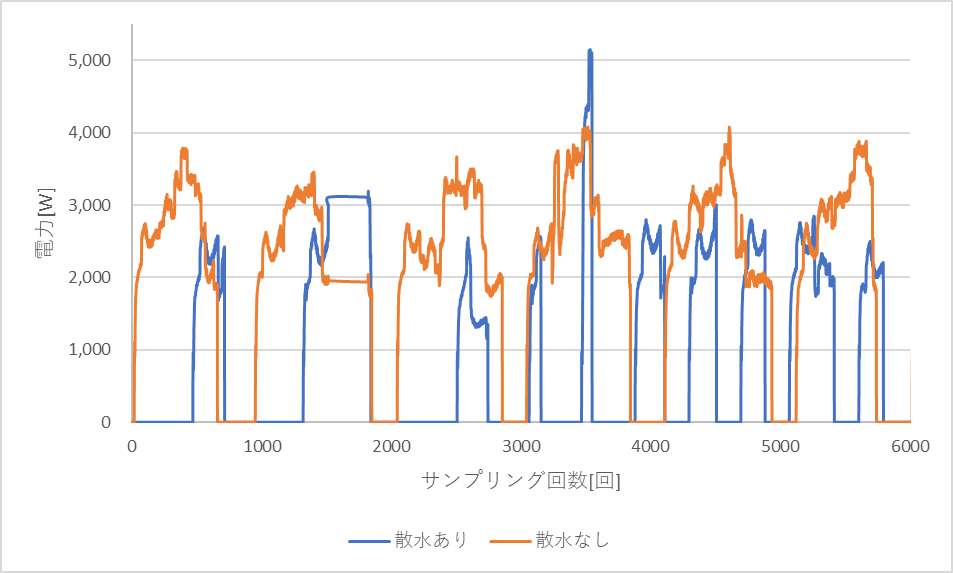
\includegraphics[width=0.9\linewidth]{img/ex1.png}
      \caption{散水の有無による電力量の比較}
      \label{fig1:compare_watering}
\end{figure*}


\begin{table*}[tbh]
  \caption{エアコン冷房時 電気代}
  \label{table:aircon}
  \centering
  \begin{tabular}{lrrrr}
    エアコン6畳タイプ & 最小消費電力 & 最大消費電力 & 期間消費電力量 & 1時間の電気代 \\
     & [W] & [W] & [Wh] & [円] \\
    \hline \hline
    DAIKIN AN22YRS-W & 115 & 960 & 630 & 17.0 \\
    Panasonic CU-X221D & 110 & 920 & 586 & 15.8 \\
    SHARP AY-N22X & 130 & 810 & 578 & 15.6 \\
    三菱電機 MSZ-ZW2221 & 105 & 850 & 594 & 16.0 \\
    日立 RAC-X22L & 115 & 880 & 555 & 15.0 \\
    \hline
  \end{tabular}
\end{table*}


\subsection{目的}\label{purpose}
\subsecref{background} より, 室外機において散水システムの導入が効果的であるという事が分かった. 
そこで本研究では, 散水システムの導入に伴い自作散水システムや市販の機器など様々な条件で比較を行い, 
電気代および水道代とのコストバランスを考慮しながら, 最適な

\section{調査内容}\label{sec2}

\subsection{DIY}\label{subsec:apriltag}

\subsection{計測}\label{subsec:tag_pos}



\section{結果}\label{sec3}

\section{考察}


\section{結論}


%参考文献
\begin{thebibliography}{99}
\bibitem{temp_osaka}
国土交通省, 気象庁, 大阪府 日最高気温の月平均値, 
\url{https://www.data.jma.go.jp/obd/stats/etrn/view/monthly_s3.php?prec_no=62&block_no=47772&year=&month=&day=&view=a2}\vspace{2mm}

\bibitem{temp_osaka2}
George's Web Sites, 大阪府-大阪市の気温に関する統計情報, 
\url{http://www.tvg.ne.jp/george/weather/gw_stat_temp.html?city=oosaka}\vspace{2mm}

\bibitem{temp_osaka3}
A-PLAT 気候変動適応プラットフォーム, 気候変動の観測・予測データ, 大阪府観測データ, 
\url{https://adaptation-platform.nies.go.jp/map/Osaka/index_past.html}\vspace{2mm}
\end{thebibliography}
%
%
%
\end{document}